% !TEX program = pdflatex
\documentclass[aspectratio=169]{beamer}

% --- Theme & packages --------------------------------------------------------
\usetheme[numbering=fraction]{metropolis}
\usepackage{amsmath,amssymb,bm}
\usepackage{booktabs,array}
\usepackage{graphicx}
\usepackage{multirow}
\usepackage{xcolor}
\usepackage{hyperref}
\hypersetup{colorlinks,urlcolor=blue,linkcolor=.,citecolor=.}
\usepackage{tikz}
\usetikzlibrary{positioning,fit,arrows.meta,calc,shapes.geometric}
\usepackage{siunitx}
\sisetup{round-mode=places,round-precision=2}
\usepackage{algorithm}
\usepackage{algorithmic}
\usepackage{inconsolata}
\usetikzlibrary{decorations.pathreplacing}

% --- Colors ------------------------------------------------------------------
\definecolor{Muted}{RGB}{110,110,110}
\definecolor{Highlight}{RGB}{200,50,50}
\definecolor{Blue}{RGB}{50,100,200}
\definecolor{Green}{RGB}{50,150,80}

% --- Typography & spacing ----------------------------------------------------
\setbeamertemplate{itemize items}[circle]
\setbeamertemplate{enumerate items}[circle]
\setbeamertemplate{blocks}[rounded][shadow=false]
\setbeamertemplate{footline}[frame number]
\setbeamertemplate{navigation symbols}{}

% --- Handy macros ------------------------------------------------------------
\newcommand{\takeaway}[1]{\begin{block}{}#1\end{block}}
\newcommand{\E}{\mathbb{E}}
\newcommand{\Var}{\mathrm{Var}}
\newcommand{\neff}{n_{\mathrm{eff}}}
\newcommand{\ghat}{\hat g_t}
\newcommand{\gtrue}{g_t}
\newcommand{\rhat}{\hat r_t}

\newcommand{\SectionSlide}[1]{%
  {\setbeamertemplate{footline}{}%
   \begin{frame}[plain,noframenumbering]
     \vfill
     \begin{center}
       {\Large\bfseries \insertsection}\\[4pt]
       {\normalsize\color{Muted} #1}
     \end{center}
     \vfill
   \end{frame}}}

% --- Metadata ----------------------------------------------------------------
\title{Adaptive Update Scaling for On-Policy RL}
\author{Runhan Yang}
\institute{CUHK--Shenzhen, SLAI}
\date{Research Meeting\\ 2026.05.07}

\begin{document}

\begin{frame}
  \titlepage
\end{frame}

\begin{frame}{Outline}
  \tableofcontents
\end{frame}

% ============================================================================
\section{Motivation}

\begin{frame}{Problem Setup: Synchronous RLVR Policy Optimization}
\small

\textbf{RLVR training objective}

\[
J(\theta)
=
\mathbb{E}_{x\sim\mathcal D,\,y\sim\pi_\theta(\cdot|x)}
\!\left[
R(x,y)
\right].
\]

{\footnotesize\color{Muted}
\(x\): prompt,\quad
\(y\): response,\quad
\(R(x,y)\): verifier reward.
}


\textbf{Synchronous PPO/GRPO update}

At step \(t\), collect a fresh on-policy rollout batch:
\[
D_t \sim \pi_{\theta_t}.
\]

Estimate a policy-update direction:
\[
\hat g_t \approx \nabla J(\theta_t).
\]

Apply one optimizer step:
\[
\theta_{t+1}
=
\theta_t
+
\alpha_t \hat g_t .
\]

\end{frame}


\begin{frame}{The RL Objective Is an Expectation, But We Only See Samples}
\small

Although \(J(\theta)\) is defined as an expectation over model-generated responses,
we cannot evaluate it exactly:
\[
J(\theta)
=
\mathbb{E}_{x\sim\mathcal D,\; y\sim\pi_\theta(\cdot|x)}
\left[
R(x,y)
\right].
\]


In fact, evaluating this expectation requires considering every possible responses:
\[
  y \in \mathcal Y(x),
  \qquad
  |\mathcal Y(x)| \text{ is enormous.}
\]


So in practice, PPO/GRPO uses a finite rollout batch:
\[
  D_t=\{(x_i,y_i)\}_{i=1}^{n},
  \qquad
  y_i\sim\pi_{\theta_t}(\cdot|x_i).
\]

This gives only a sampled estimate of the true update direction:
\[
  \hat g_t
  =
  g_t+\epsilon_t .
\]

\begin{center}
\large
\textbf{Finite on-policy sampling introduces gradient-estimation error.}
\end{center}

\end{frame}


\begin{frame}{Why Gradient Noise Changes During RL Training}
\small

At step \(t\), the update direction is estimated from on-policy samples:
\[
  D_t=\{(x_i,y_i)\}_{i=1}^n,
  \qquad
  y_i\sim\pi_{\theta_t}(\cdot|x_i).
\]

So the gradient estimate can be written as
\[
  \hat g_t = g_t+\epsilon_t,
\]
where \(\epsilon_t\) is the finite-sample error from the rollout batch.

\vspace{0.8em}

Unlike supervised learning, the sampling distribution is not fixed:
\[
  \pi_{\theta_t}
  \longrightarrow
  \pi_{\theta_{t+1}}.
\]

\vspace{0.8em}

Therefore the noise distribution also changes:
\[
  \epsilon_t \sim \mathcal E(\pi_{\theta_t}),
  \qquad
  \mathbb E\|\epsilon_t\|^2 = v_t .
\]



\end{frame}


\begin{frame}{Fixed LR Ignores Changing Estimation Quality}
\small

A fixed learning rate applies the same update scale:
\[
  \theta_{t+1}
  =
  \theta_t+\alpha\hat g_t,
  \qquad
  \alpha \text{ is constant.}
\]

\vspace{0.8em}

But the gradient estimate has changing signal-to-noise structure:
\[
  \hat g_t=g_t+\epsilon_t,
  \qquad
  \mathbb E\|\epsilon_t\|^2=v_t .
\]

\vspace{0.8em}

If \(v_t\) is small, the sampled direction is reliable and can support a larger update.

If \(v_t\) is large, the same update scale may amplify sampling noise.

\vspace{0.8em}

So fixed LR creates a mismatch:
\[
  \text{constant update scale}
  \quad\text{vs.}\quad
  \text{changing batch reliability}.
\]

\end{frame}


\begin{frame}{Fixed LR Sweep: Optimization and Validation}
\small

\begin{center}
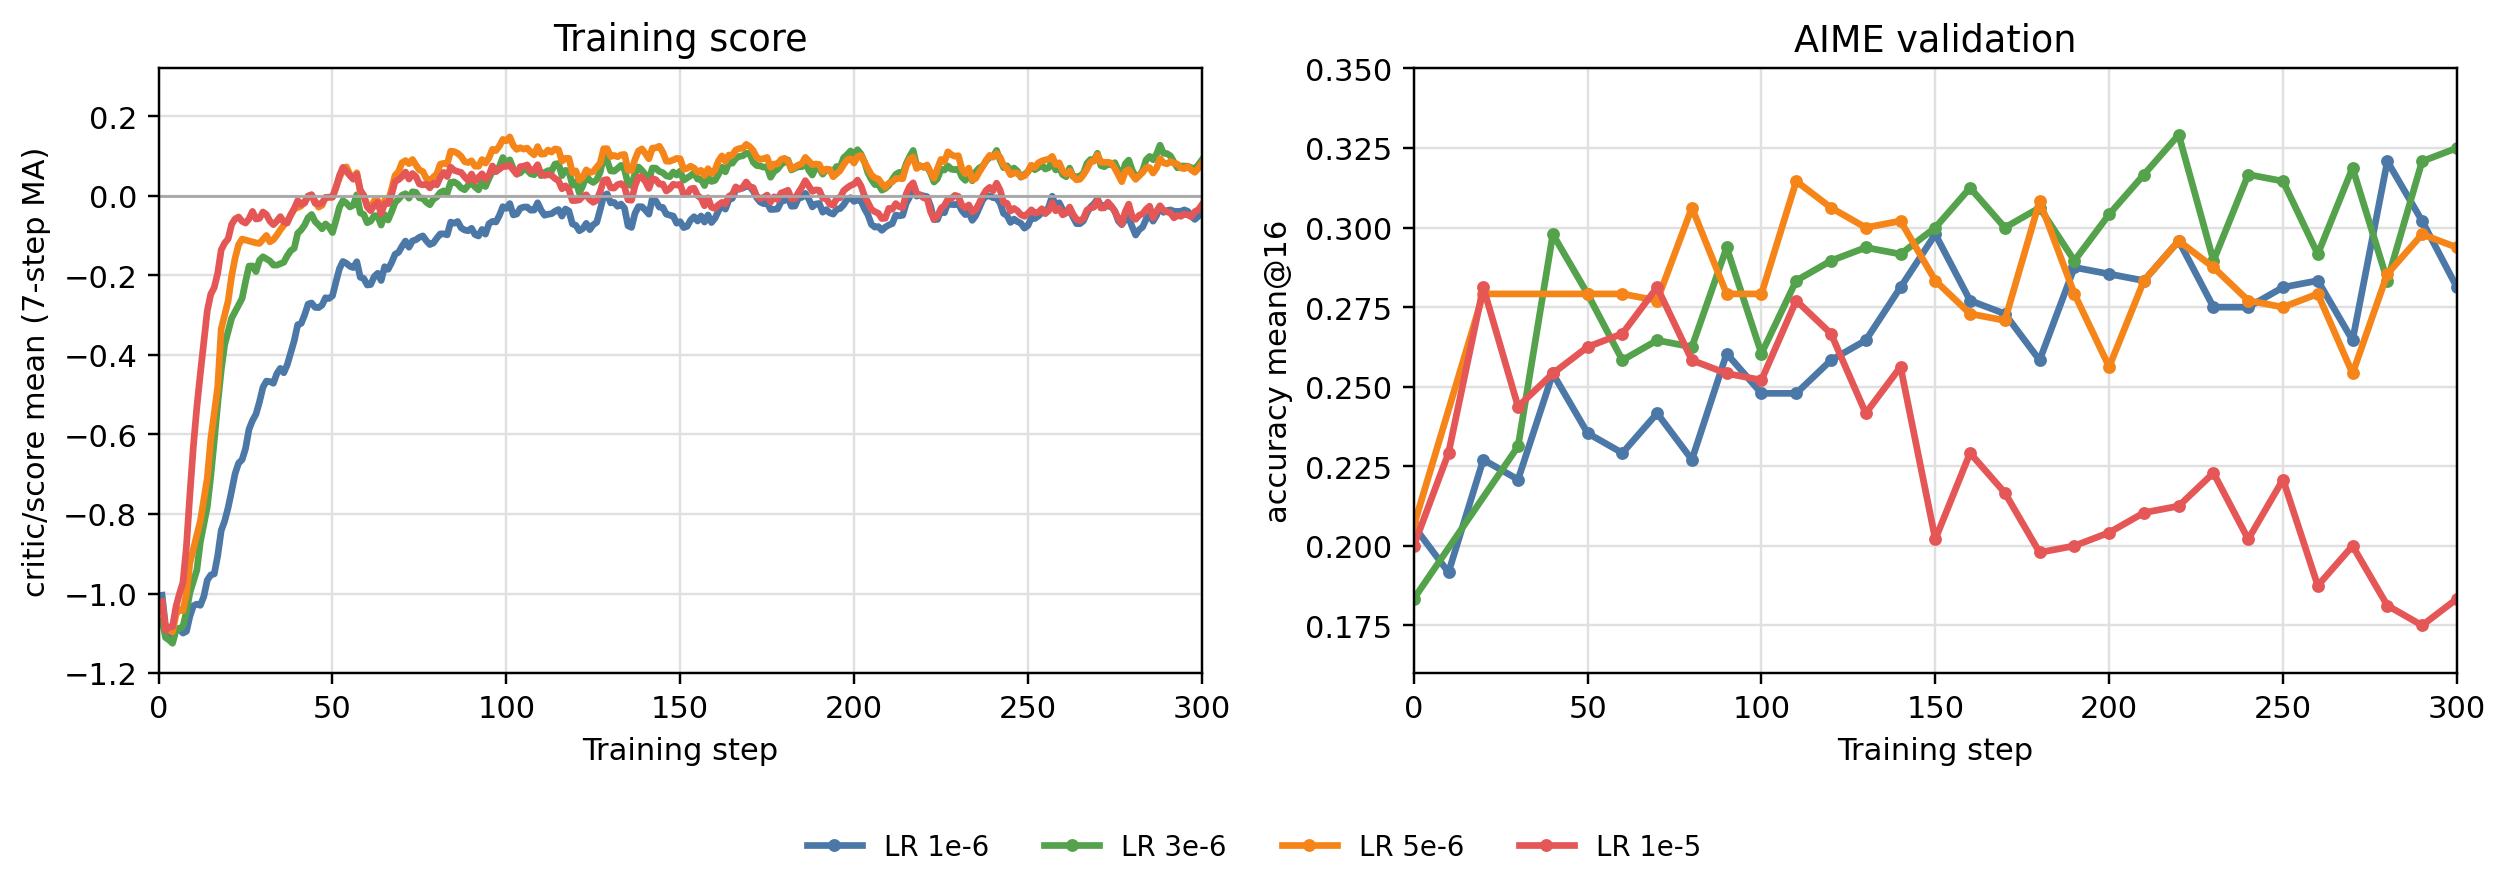
\includegraphics[width=0.92\linewidth]{figures/fixed_lr_sweep_objective_aime.png}
\end{center}

\vspace{-0.2em}

\begin{itemize}
  \item \(1\mathrm{e}{-5}\) peaks early in both training score and AIME, then regresses.
  \item \(3\mathrm{e}{-6}\) gives the best final AIME among fixed-LR runs.
  \item The high-LR run degrades on both the empirical optimization objective and validation.
\end{itemize}

\end{frame}


\begin{frame}{From Fixed LR Limitation to LR Scheduling}
\small

The fixed-LR sweep shows a phase trade-off:
\[
\text{small LR: stable but slow},
\qquad
\text{large LR: fast early but unstable later}.
\]

\vspace{0.8em}

This suggests that no single fixed learning rate is ideal across all training phases.

\vspace{0.8em}

In on-policy RL, the quality of the sampled update direction changes during training:
\[
  \hat g_t = g_t + \epsilon_t,
  \qquad
  \mathbb E\|\epsilon_t\|^2 = v_t .
\]

\vspace{0.8em}

So the next question is:

\[
  \textbf{How should we schedule } \alpha_t \textbf{ over training?}
\]

\vspace{0.8em}


\end{frame}



\section{Optimization Criterion}

\begin{frame}{From Smoothness to Expected Improvement}
\small

Consider one stochastic policy update:
\[
  \theta_{t+1}=\theta_t+\alpha \hat g_t .
\]

For a locally \(L\)-smooth objective,
\[
  J(\theta_{t+1})-J(\theta_t)
  \ge
  \alpha g_t^\top \hat g_t
  -
  \frac{L}{2}\alpha^2\|\hat g_t\|^2 ,
\]
where \(g_t=\nabla J(\theta_t)\).

\vspace{0.7em}

Taking expectation over finite-batch sampling:
\[
  \mathbb E[g_t^\top \hat g_t]=\|g_t\|^2 .
\]

\vspace{0.6em}

Also,
\[
  \mathbb E\|\hat g_t\|^2
  =
  \|g_t\|^2
  +
  \mathbb E\|\hat g_t-g_t\|^2 .
\]

\end{frame}


\begin{frame}{Signal and Finite-Sample Noise}
\small

Let the stochastic update be
\[
  \hat g_t = g_t + \epsilon_t,
  \qquad
  \mathbb{E}[\epsilon_t]=0.
\]

\vspace{0.6em}

Define the finite-sample noise level:
\[
  v_t
  =
  \mathbb{E}\|\epsilon_t\|^2
  =
  \mathbb{E}\|\hat g_t-g_t\|^2 .
\]

\vspace{0.8em}

Then the expected one-step improvement becomes
\[
  \mathbb{E}[\Delta J_t]
  \gtrsim
  \alpha \|g_t\|^2
  -
  \frac{L}{2}\alpha^2
  \left(
    \|g_t\|^2+v_t
  \right).
\]

\vspace{0.9em}


\end{frame}


\begin{frame}{Optimal LR Contains a Signal Fraction}
\small

The lower bound is a quadratic function of \(\alpha\):
\[
  f(\alpha)
  =
  \alpha A
  -
  \frac{L}{2}\alpha^2 B,
  \qquad
  A=\|g_t\|^2,\quad
  B=\|g_t\|^2+v_t .
\]

Taking derivative:
\[
  f'(\alpha)=A-LB\alpha .
\]

Thus
\[
  \alpha_t^*
  =
  \frac{\|g_t\|^2}
       {L(\|g_t\|^2+v_t)} .
\]

Define the signal fraction:
\[
  r_t
  =
  \frac{\|g_t\|^2}
       {\|g_t\|^2+v_t}
  \in [0,1].
\]

Then
\[
  \alpha_t^*
  =
  \frac{r_t}{L}.
\]

\end{frame}

\begin{frame}{Decomposing the Learning Rate}
\small

From the expected-improvement bound:
\[
  \alpha_t^*
  =
  \frac{\|g_t\|^2}
       {L_t\left(\|g_t\|^2+v_t\right)} .
\]

\vspace{0.4em}

{\color{Muted}
\(L_t\) is step-dependent because PPO/GRPO optimizes a sampled local surrogate
\(\widehat L_t(\theta;D_t)\).
}

\vspace{1.0em}

Define two factors:
\[
  r_t
  =
  \frac{\|g_t\|^2}
       {\|g_t\|^2+v_t},
  \qquad
  c_t
  =
  \frac{1}{L_t}.
\]

\vspace{1.0em}

Then the optimal scale becomes
\[
  \boxed{
  \alpha_t^*
  =
  c_t\, r_t
  }.
\]

\vspace{0.7em}

\begin{center}
\large
\textbf{\(r_t\): batch reliability \qquad \(c_t\): local scale}
\end{center}

\end{frame}



\section{Method}

\begin{frame}{Experimental Strategy: Isolate the \(r_t\)-Side}
\small

From the decomposition,
\[
  \alpha_t^*
  =
  c_t r_t .
\]

\vspace{0.6em}

Both factors are unknown.



\vspace{0.9em}

So in the current experiments, we first fix the scale:
\[
  c_t = c_{\mathrm{fix}},
\]
where \(c_{\mathrm{fix}}\) is selected from a preliminary LR sweep.


Then we test only the reliability-side schedule:
\[
  \alpha_t
  =
  c_{\mathrm{fix}}\, \hat r_{\mathrm{ctrl},t}.
\]



\end{frame}


\begin{frame}{Estimating \(r_t\) from Mini-Batch Splits}
\small

We want the signal fraction
\[
  r_t
  =
  \frac{\|g_t\|^2}{\|g_t\|^2+v_t},
\]
but \(g_t\) and \(v_t\) are not directly observable.

\vspace{0.8em}

In PPO/GRPO, the rollout batch is processed through mini-batches.
For each mini-batch \(M_{t,k}\), we split it into two halves:
\[
  M_{t,k}
  =
  A_{t,k}
  \cup
  B_{t,k}.
\]

\vspace{0.7em}

Each half gives a gradient estimate:
\[
  \hat g_{A,k}
  =
  g_{t,k}+\epsilon_{A,k},
  \qquad
  \hat g_{B,k}
  =
  g_{t,k}+\epsilon_{B,k}.
\]



\end{frame}


\begin{frame}{Split Agreement Estimates Signal Fraction}
\small

Assume the two half-batch noises are independent and zero-mean:
\[
  \mathbb{E}[\epsilon_{A,k}]
  =
  \mathbb{E}[\epsilon_{B,k}]
  =
  0.
\]

Then
\[
  \mathbb{E}
  \left[
    \hat g_{A,k}^{\top}\hat g_{B,k}
  \right]
  =
  \|g_{t,k}\|^2 .
\]

\vspace{0.7em}

The half-batch norms contain both signal and noise:
\[
  \mathbb{E}\|\hat g_{A,k}\|^2
  =
  \|g_{t,k}\|^2
  +
  \mathbb{E}\|\epsilon_{A,k}\|^2 .
\]

\vspace{0.8em}

So we estimate the mini-batch signal fraction by
\[
  \hat r_{t,k}
  =
  \frac{
    \hat g_{A,k}^{\top}\hat g_{B,k}
  }{
    \frac{1}{2}
    \left(
      \|\hat g_{A,k}\|^2
      +
      \|\hat g_{B,k}\|^2
    \right)
  }.
\]

\end{frame}


\begin{frame}{Mini-Batch-Level LR Control}
\small

Each mini-batch produces its own signal-fraction estimate:
\[
  \hat r_{t,k}.
\]

\vspace{0.7em}

In the base experiments, we use the current mini-batch estimate directly,
with only clipping / guards:
\[
  r_{\mathrm{ctrl},t,k}
  =
  \mathrm{clip}
  \left(
    \hat r_{t,k},
    r_{\min},
    r_{\max}
  \right).
\]

\vspace{0.8em}

The learning rate for this mini-batch update is
\[
  \alpha_{t,k}
  =
  c_{\mathrm{fix}}\,
  r_{\mathrm{ctrl},t,k}.
\]

\vspace{0.8em}

Then update with the current mini-batch gradient:
\[
  \theta
  \leftarrow
  \theta
  +
  \alpha_{t,k}\hat g^{\mathrm{upd}}_{t,k}.
\]

\vspace{0.5em}


\end{frame}


\section{Main Results}

\begin{frame}{Ablation Design: Baselines}
\small

Current experiments fix the scale term:
\[
  c_t=c_{\mathrm{fix}},
  \qquad
  \alpha_{t,k}=c_{\mathrm{fix}}\,r_{\mathrm{ctrl},t,k}.
\]

\vspace{0.7em}

So we test whether the mini-batch-level reliability schedule
\(r_{\mathrm{ctrl},t,k}\) adds value.

\vspace{0.6em}

\begin{center}
\scriptsize
\begin{tabular}{lll}
\toprule
Run family & What is matched & Question tested \\
\midrule
Best fixed LR
& LR sweep optimum
& Do we beat the tuned fixed baseline? \\
Mean-matched constant LR
& mean update scale
& Is the gain only from average LR? \\
Ours: signal fraction
& online \(r_{\mathrm{ctrl}}\)
& Does batch feedback add value? \\
\bottomrule
\end{tabular}
\end{center}

\vspace{0.4em}

{\footnotesize\color{Muted}
All run families are repeated with 3 random seeds.
}

\end{frame}


\begin{frame}{Ablation Design: Limitation}
\small

This baseline is useful, but it is not an exact counterfactual replay.

\vspace{0.8em}

In on-policy RL, changing the LR changes the next policy:
\[
  \alpha_t
  \longrightarrow
  \theta_{t+1}.
\]

\vspace{0.6em}

Then the next rollout batch also changes:
\[
  D_{t+1}
  \sim
  \pi_{\theta_{t+1}}.
\]

\vspace{0.8em}

\begin{center}
\large
\textbf{So we cannot exactly replay the same sampled training landscape under a different LR schedule.}
\end{center}

\vspace{0.6em}

{\footnotesize\color{Muted}
The mean-matched constant baseline matches average update scale,
not the exact on-policy data path.
}

\end{frame}


\begin{frame}{1.5B Result: Mini-Batch Reliability Schedule Helps}
\small

\begin{center}
\scriptsize
\begin{tabular}{lrrrr}
\toprule
Family & Tail train obj. & Best avg5 & Final avg5 & Drop \\
\midrule
Ours: signal fraction & \textbf{0.115} & \textbf{0.3443} & \textbf{0.3443} & \textbf{0.0000} \\
Best fixed LR \(3\mathrm{e}{-6}\) & 0.090 & \textbf{0.3445} & 0.3404 & -0.0041 \\
Mean-matched const. \(3.10\mathrm{e}{-6}\) & 0.068 & 0.3328 & 0.3322 & -0.0005 \\
\bottomrule
\end{tabular}
\end{center}

\vspace{0.4em}

{\footnotesize\color{Muted}
avg5 = AIME, AIME2025, GPQA, MINERVA, OLYMPIAD\_BENCH.
Tail train obj. = mean \(\mathrm{critic/score/mean}\) over the last 20 train steps.
}

\vspace{0.7em}

\begin{itemize}
  \item Ours is better not only on validation avg5, but also on the sampled training objective.
  \item Best fixed LR reaches a similar peak, but has lower final avg5 and lower tail train objective.
  \item The mean-matched constant is lower, so average LR alone is insufficient.
\end{itemize}

\end{frame}

\begin{frame}{Actual LR Scale: Online vs Fixed-LR Baselines}
\small

\begin{center}
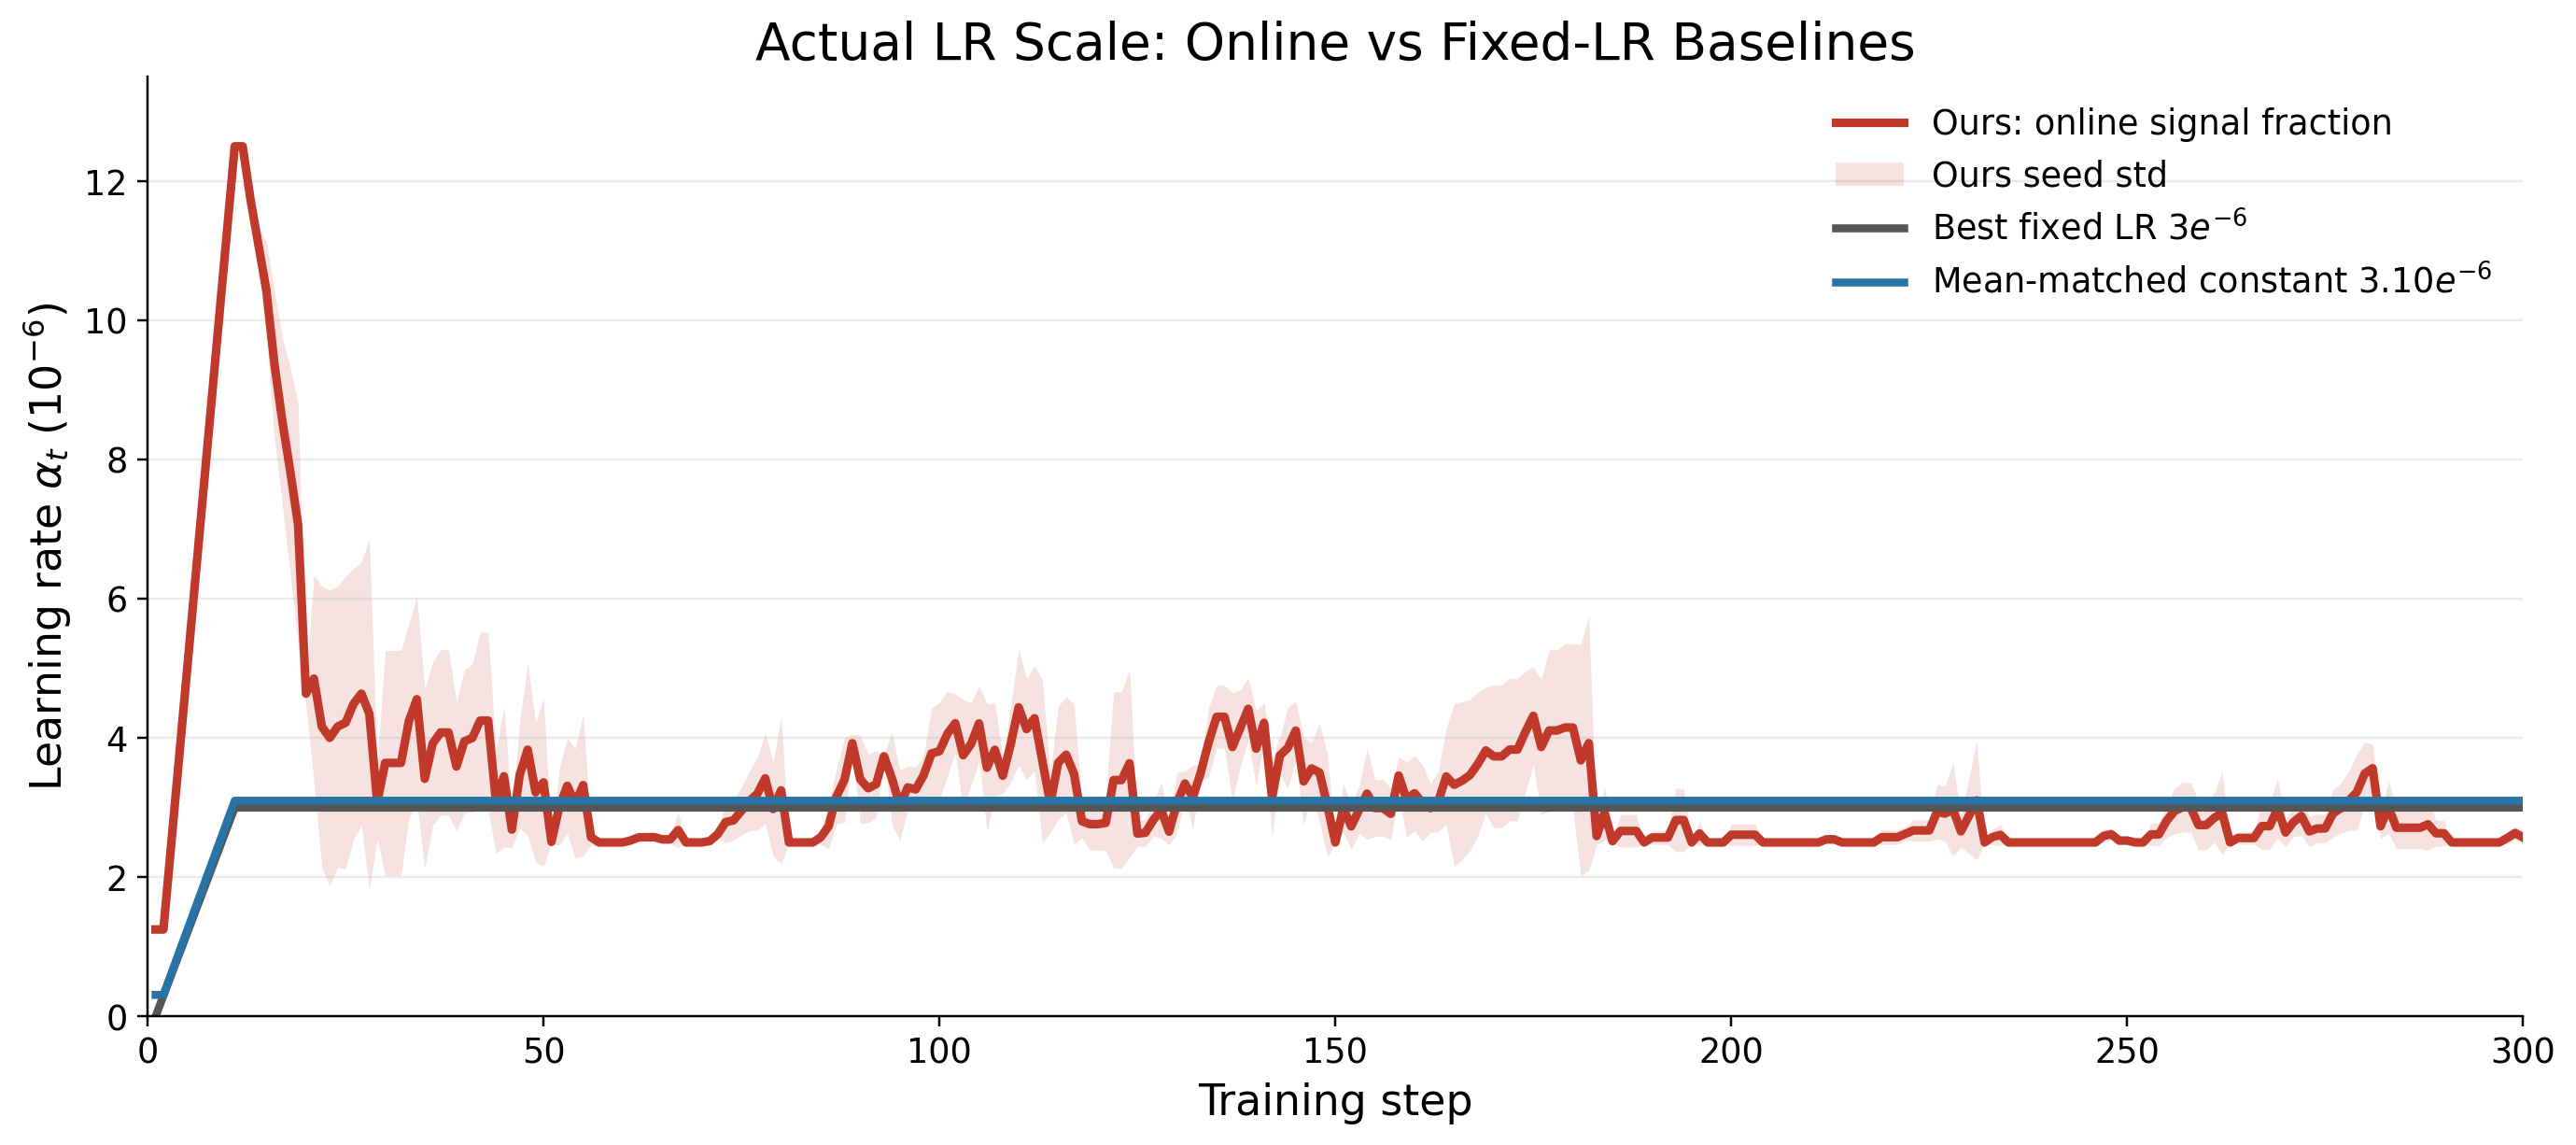
\includegraphics[width=0.8\linewidth]{figures/main_alpha_schedules_1p5b.png}
\end{center}

\vspace{-1.0em}

\begin{itemize}
  \item The online controller uses a noisy, non-monotone LR trajectory.
  \item \(3\mathrm{e}{-6}\) is the tuned fixed-LR baseline from the sweep.
  \item Mean-matched constant tests whether the result is only due to average LR scale.
\end{itemize}

\end{frame}




\section{Controller Analysis}

\begin{frame}{Finding: Raw Split Signal Is Noisy}
\small

Raw split agreement is weak:
\[
  \Pr(\hat g_A^\top \hat g_B>0)\approx 55\%.
\]

\vspace{0.7em}

This suggests:
\[
  \hat r_{t,k}
  =
  \frac{\hat g_A^\top \hat g_B}
       {\frac12(\|\hat g_A\|^2+\|\hat g_B\|^2)}
\]
is not a precise SNR estimator.

\vspace{0.8em}

\textbf{Working hypothesis:}
\[
  \hat r_{t,k}
  \text{ is a noisy reliability proxy.}
\]

\vspace{0.8em}

So we tested whether lower-bandwidth controllers can turn this weak signal into a stable LR schedule.

\end{frame}


\begin{frame}{Are There Other Reliable Proxies?}
\small

We also checked standard RL training diagnostics:

\vspace{0.4em}

\begin{center}
\scriptsize
\begin{tabular}{lll}
\toprule
Signal & What it measures & Limitation for our question \\
\midrule
Grad norm & update magnitude & not estimator reliability \\
KL / ratio tail & policy movement / IS risk & can stay small during performance drop \\
Response length & generation behavior & confounded with reward format and overlong penalty \\
Entropy & policy concentration & useful state signal, but not a direct LR rule \\
Reward / advantage stats & batch outcome variation & task-dependent and sparse \\
\bottomrule
\end{tabular}
\end{center}

\vspace{0.7em}

These signals are useful diagnostics, but none directly answers:
\[
  \textbf{How reliable is the current batch gradient direction?}
\]


\large
\textbf{So we keep split-batch alignment as the main reliability proxy, but treat it as noisy.}

\end{frame}


\begin{frame}{First Attempts: Lower-Bandwidth Controllers}
\small

\textbf{Goal:}
make the noisy \(r_t\) signal enter the LR controller more slowly or more safely.


\begin{center}
\tiny
\begin{tabular}{llrrrr}
\toprule
Variant & Design & Tail obj. & Best & Final & Drop \\
\midrule
Current B
& clipped mini-batch \(r_t\) controller
& 0.115 & 0.3443 & 0.3443 & 0.0000 \\
\texttt{alpharlim0.05}
& \(\alpha_t\in[0.95,1.05]\alpha_{t-1}\)
& 0.143 & 0.3428 & 0.3403 & -0.0025 \\
\texttt{slowema\_0.95}
& EMA retention \(0.95\)
& 0.143 & 0.3483 & 0.3408 & -0.0075 \\
\texttt{slowema\_0.98}
& EMA retention \(0.98\)
& 0.086 & 0.3378 & 0.3240 & -0.0138 \\
\texttt{windowr\_w5}
& mean of latest 5 valid \(r_t\)
& \textbf{0.160} & 0.3309 & 0.3206 & -0.0103 \\
\texttt{windowr\_w10}
& mean of latest 10 valid \(r_t\)
& 0.150 & \textbf{0.3527} & \textbf{0.3481} & -0.0046 \\
\bottomrule
\end{tabular}
\end{center}

\vspace{0.4em}

{\footnotesize\color{Muted}
Tail obj. = mean \(\mathrm{critic/score/mean}\) over the last 20 train steps.
}

\vspace{0.4em}

\begin{itemize}
  \item Slow EMA and alpha-rate limit reduce high-frequency controller motion, but do not clearly beat B.
  \item W10 gives the strongest positive signal, suggesting temporal aggregation can help.
  \item The next question is whether W10 is robust across repeated seeds.
\end{itemize}

\end{frame}

\begin{frame}{Lower-Bandwidth Controllers: LR Trajectories}
\small

\begin{center}
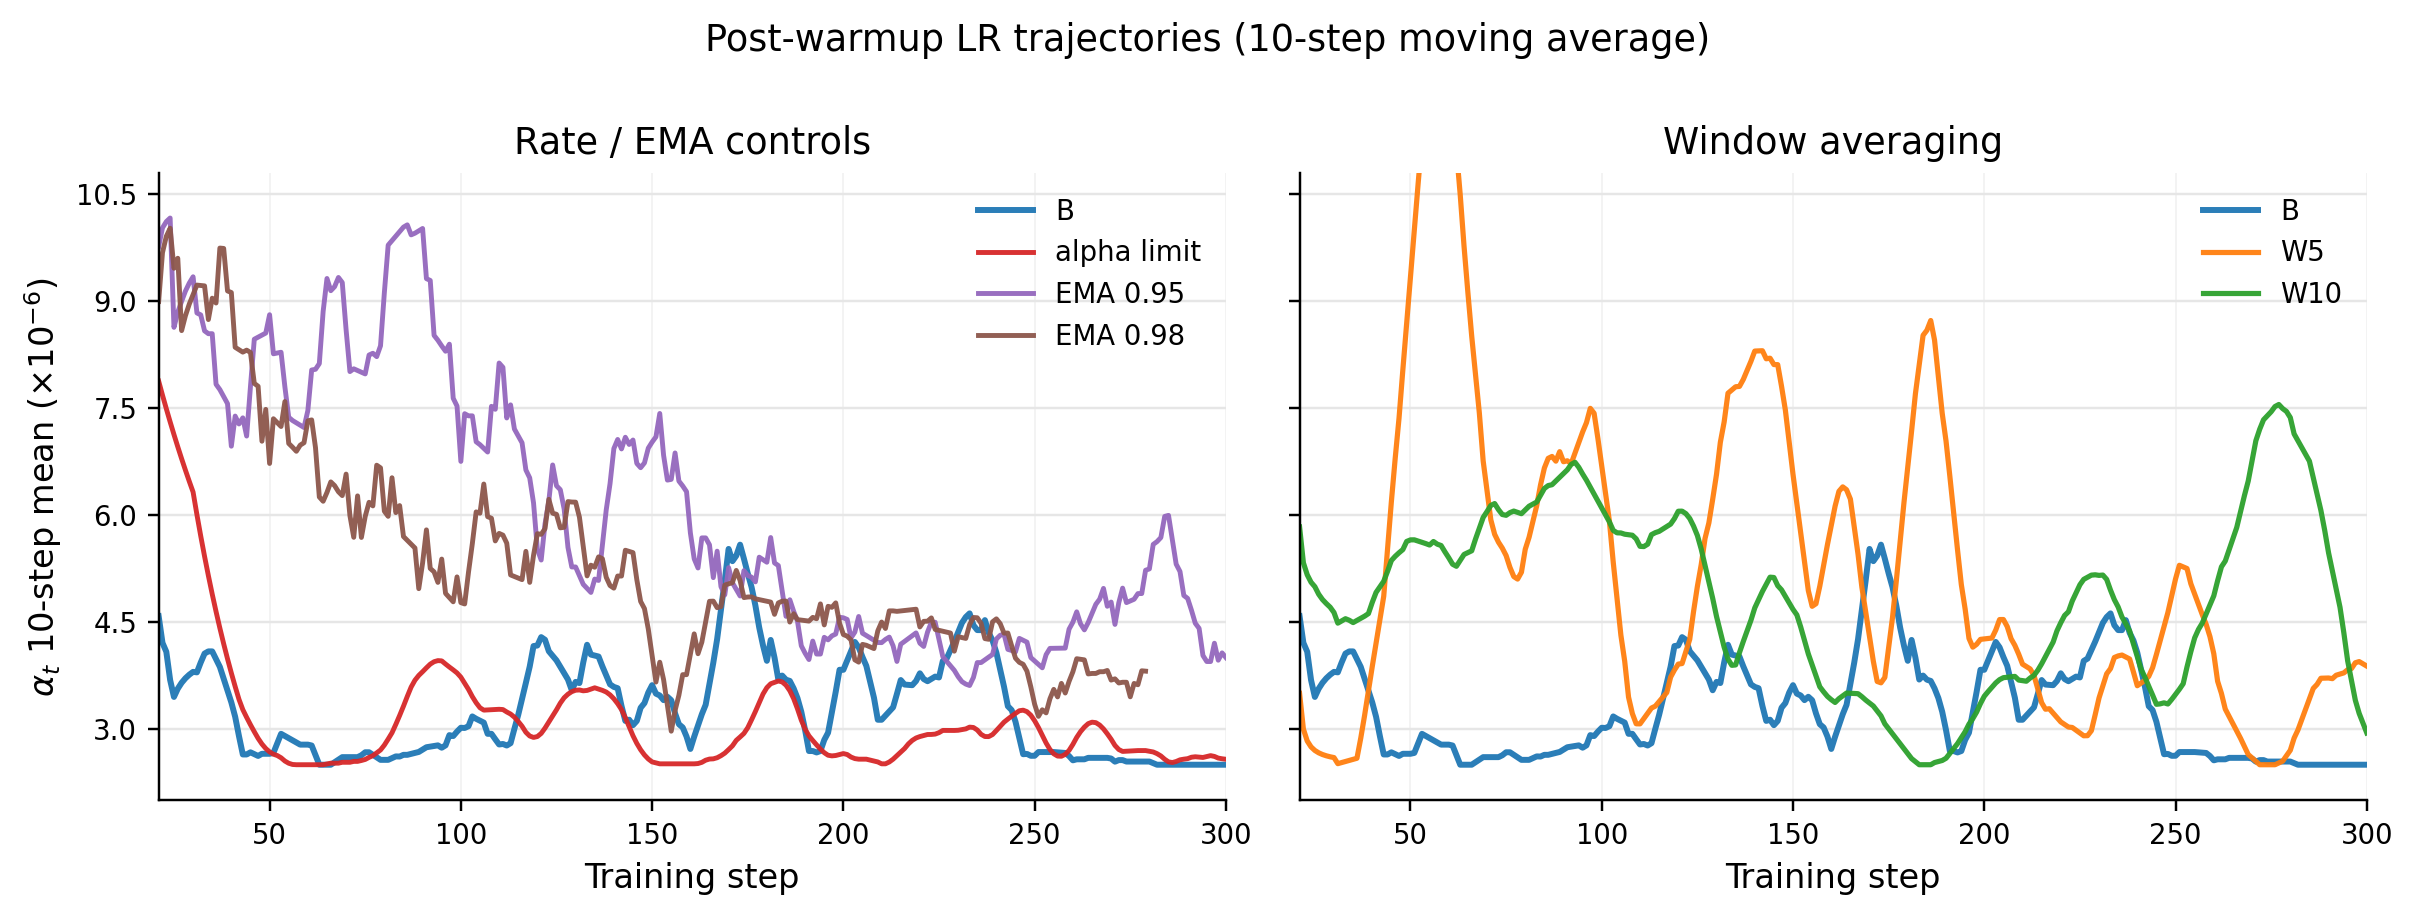
\includegraphics[width=0.95\linewidth]{figures/lower_bandwidth_alpha_trajectories.png}
\end{center}

\vspace{-1.5em}

\begin{itemize}
  \item These are new controllers, not smoothed versions of the B trajectory.
  \item Slow EMA keeps a large delayed LR response, which may explain its weak final stability.
  \item Window averaging changes the trajectory more substantially; W10 is the most promising variant.
\end{itemize}

\end{frame}


\begin{frame}{W10: Strongest Positive Signal}
\small

W10 replaces the per-step \(r_t\) input with a windowed average:
\[
  r^{(10)}_t
  =
  \frac{1}{|{\cal W}_t|}
  \sum_{i\in{\cal W}_t}
  \hat r_i,
  \qquad
  \alpha_t=c_{\mathrm{fix}}r^{(10)}_t .
\]

\vspace{0.5em}

\begin{center}
\scriptsize
\begin{tabular}{lrrrr}
\toprule
Run group & Tail obj. & Best avg5 & Final avg5 & Drop \\
\midrule
W10 seed0 & 0.117 & 0.3456 & 0.3419 & -0.0037 \\
W10 seed1 & \textbf{0.194} & \textbf{0.3624} & \textbf{0.3600} & -0.0024 \\
W10 seed42 rerun & 0.136 & 0.3500 & 0.3423 & -0.0077 \\
\midrule
Mean of these 3 runs & 0.150 & 0.3527 & 0.3481 & -0.0046 \\
\bottomrule
\end{tabular}
\end{center}

\vspace{0.4em}

\begin{itemize}
  \item W10 is the first low-bandwidth variant with a clear positive signal.
  \item This suggests the useful part of split-batch alignment may be low-frequency.
  \item But we still need to test whether this holds under repeated seeds.
\end{itemize}

\end{frame}

\begin{frame}{W10 Repeat Reveals a Failure Case}
\small

\textbf{W10 seed2: good early trajectory, then late collapse.}

\begin{center}
\scriptsize
\begin{tabular}{lrrrrrrr}
\toprule
Step & Train obj. & avg5 & AIME & AIME25 & GPQA & MINERVA & OLYMP. \\
\midrule
120 & 0.0247 & \textbf{0.3350} & 0.3125 & 0.2313 & 0.3450 & \textbf{0.2781} & \textbf{0.5081} \\
240 & -0.0453 & 0.3185 & 0.2979 & 0.2125 & 0.3444 & 0.2469 & 0.4906 \\
300 & 0.0081 & 0.2877 & 0.2750 & 0.2042 & \textbf{0.3700} & 0.1894 & 0.4000 \\
\bottomrule
\end{tabular}
\end{center}

\vspace{0.3em}

{\footnotesize\color{Muted}
Train obj. = \(\mathrm{critic/score/mean}\) at the same training step.
}

\vspace{0.4em}

\begin{itemize}
  \item The collapse is not uniform: GPQA keeps improving.
  \item The main late drops are MINERVA and OLYMPIAD.
  \item So W10 can extract useful low-frequency signal, but windowing alone does not guarantee stability.
\end{itemize}

\end{frame}


\begin{frame}{Diagnosis: W10 Can Still Overshoot Alpha}
\small

In seed2, W10 creates a suspicious LR spike after step 200:

\begin{center}
\scriptsize
\begin{tabular}{lrrrr}
\toprule
Stage & mean \(\alpha_t\) & mean \(r_{\mathrm{window}}\) & entropy & KL max \\
\midrule
51--120 & \(4.23\mathrm{e}{-6}\) & 0.0169 & 0.385 & 0.90 \\
121--200 & \(4.59\mathrm{e}{-6}\) & 0.0183 & 0.392 & 0.99 \\
201--240 & \(8.64\mathrm{e}{-6}\) & 0.0346 & 0.218 & 2.49 \\
241--270 & \(1.02\mathrm{e}{-5}\) & 0.0406 & 0.580 & 0.98 \\
\bottomrule
\end{tabular}
\end{center}

\vspace{0.6em}

\begin{itemize}
  \item Window averaging filters single-step noise, but can still be fooled by a short positive burst.
  \item Once \(r_{\mathrm{window}}\) rises, \(\alpha_t=c_{\mathrm{fix}}r_{\mathrm{window}}\) can become too aggressive.
  \item Therefore W10 needs a safeguard on the LR trajectory itself.
\end{itemize}

\end{frame}

\begin{frame}{W10 + Alpha Rate Limit}
\small

\textbf{Keep the useful low-frequency signal:}
\[
  r_{\mathrm{window},t}
  =
  \mathrm{mean}
  \left(
    \hat r_{t-W+1},\ldots,\hat r_t
  \right),
  \qquad
  W=10.
\]

\vspace{0.6em}

\textbf{But prevent sudden LR jumps:}
\[
  \alpha^{\mathrm{raw}}_t
  =
  c_{\mathrm{fix}}r_{\mathrm{window},t},
  \qquad
  \alpha_t
  =
  \mathrm{clip}
  \left(
    \alpha^{\mathrm{raw}}_t,\,
    0.95\alpha_{t-1},\,
    1.05\alpha_{t-1}
  \right).
\]

\vspace{0.8em}

\textbf{What this tests}

\begin{itemize}
  \item W10 + alpha limit tests whether W10's failure is caused by LR overshoot.
  \item It does not by itself separate low-frequency signal from larger mean LR.
  \item The key case is seed2: can we keep the early gain without the late collapse?
\end{itemize}

\end{frame}

\begin{frame}{W10 + Alpha Limit: Suppress LR Spike}
\small

\begin{center}
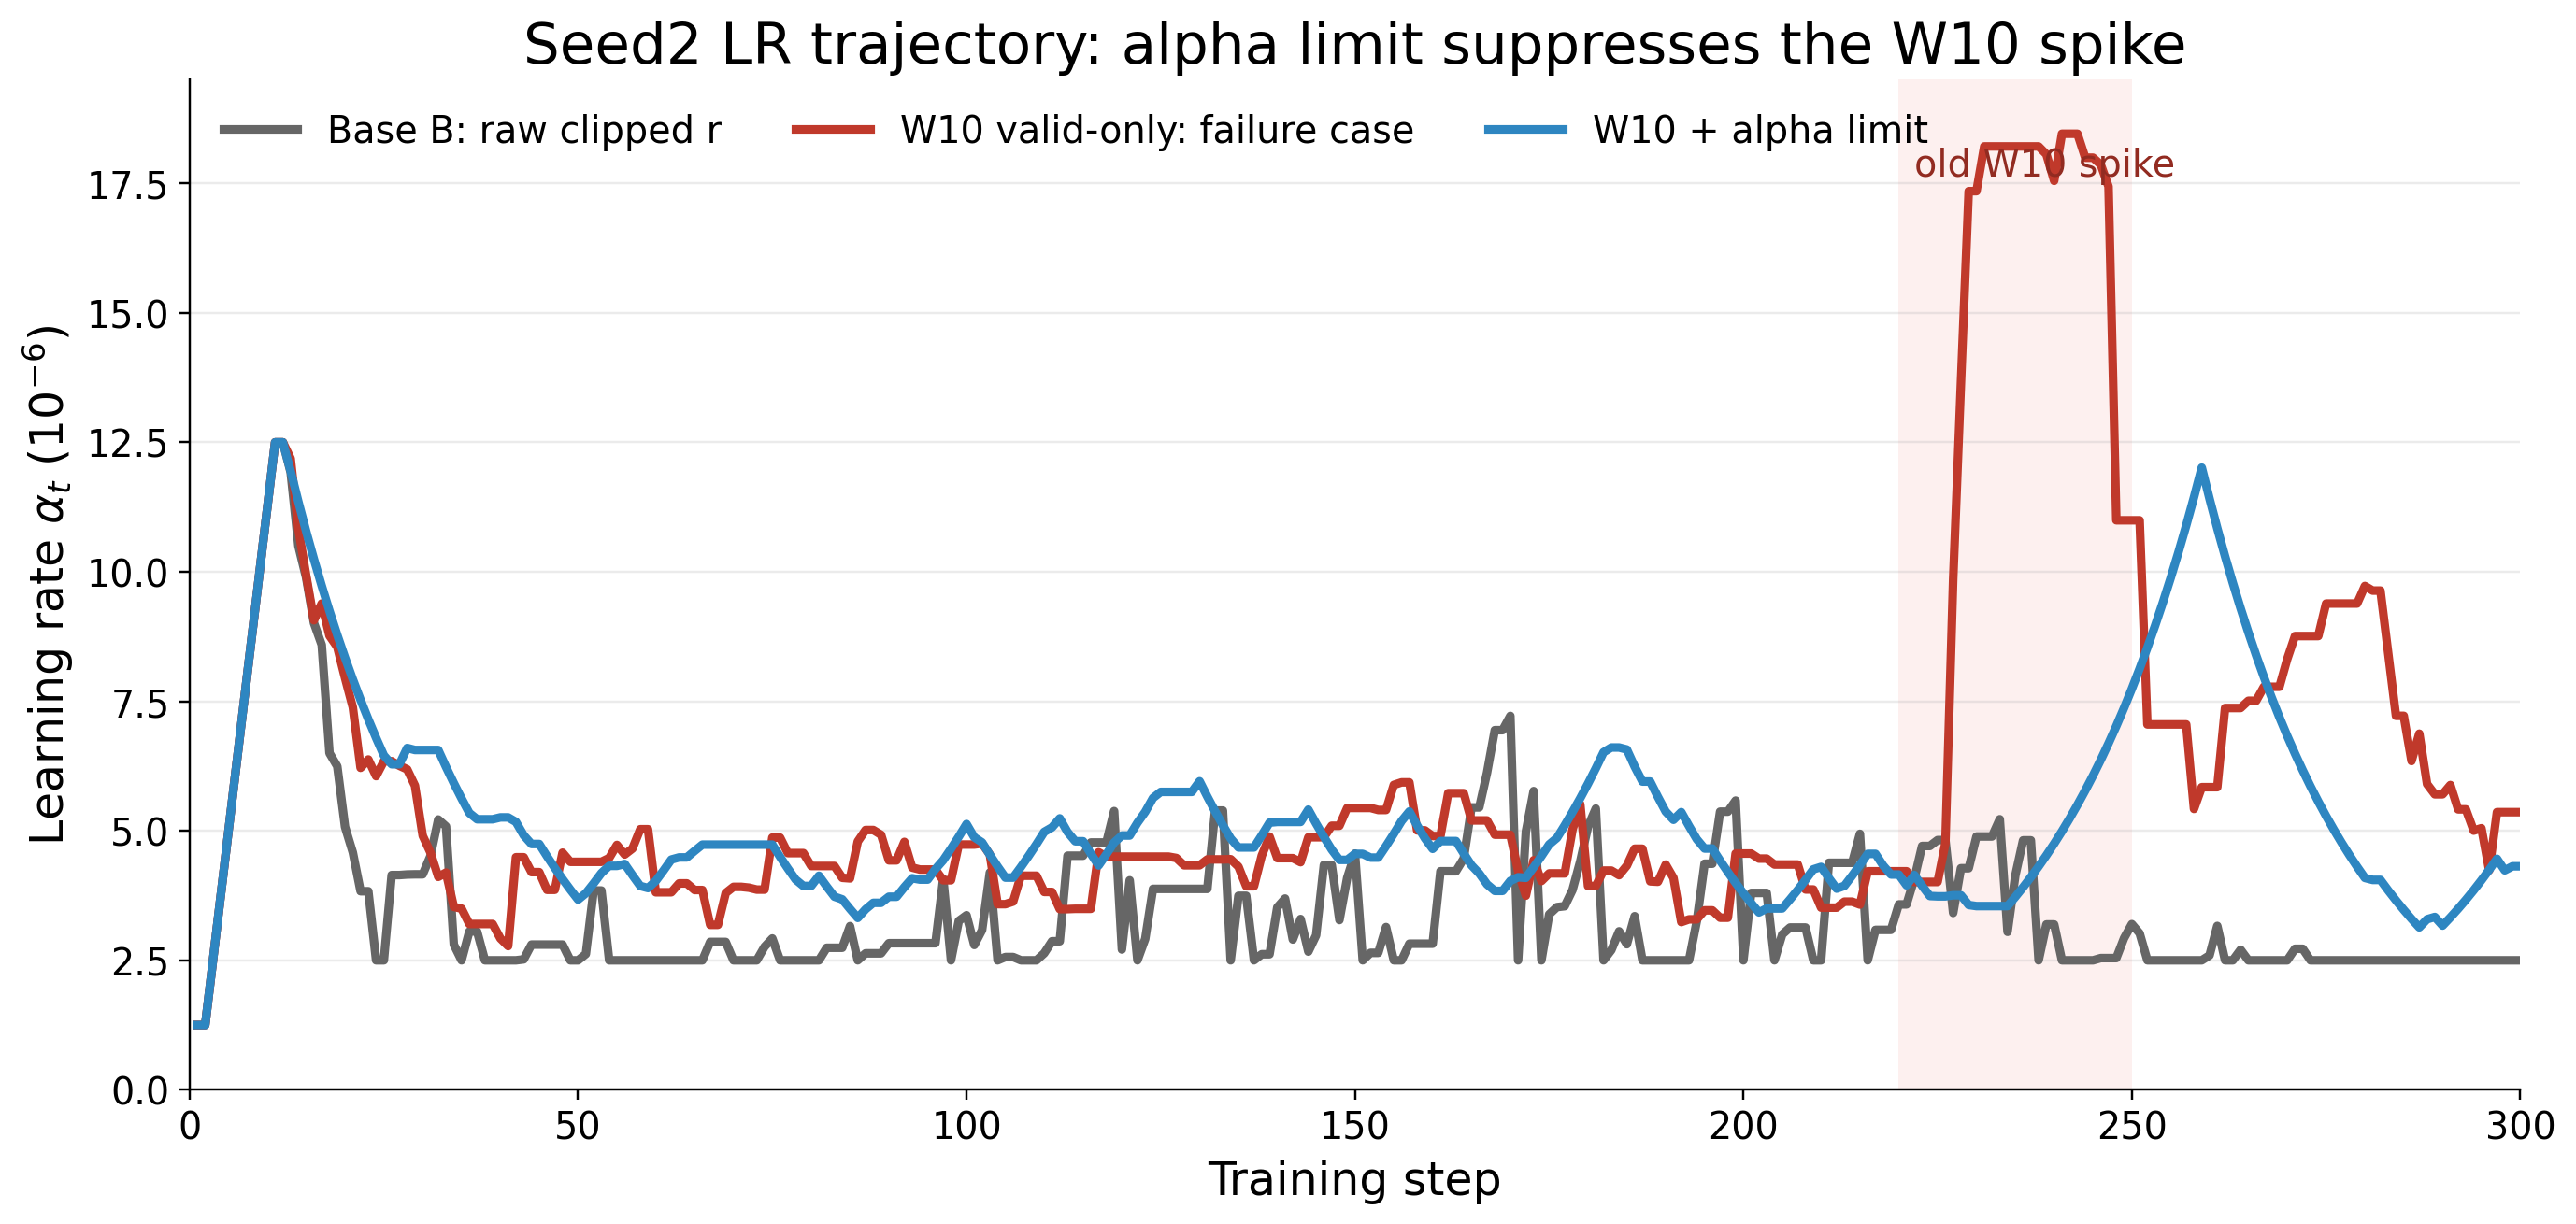
\includegraphics[width=0.8\linewidth]{figures/w10_seed2_alpha_limit.png}
\end{center}

\vspace{-1.0em}

\begin{itemize}
  \item Old W10 seed2 shows a large LR spike around steps 230--250.
  \item Alpha limiting suppresses the abnormal jump and keeps the LR tail smaller.
  \item This supports the diagnosis that W10's seed2 failure is partly an LR-overshoot problem.
\end{itemize}

\end{frame}


\begin{frame}{Remaining Issue: Valid-Only W10 Raises LR Scale}
\small

The current W10 controller stores only valid positive split signals:
\[
  \hat r_i \in {\cal W}_t
  \quad\text{only if}\quad
  \hat g_A^\top\hat g_B>0 .
\]

\vspace{0.6em}

Then the controller averages this selected window:
\[
  r^{(10)}_t
  =
  \frac{1}{|{\cal W}_t|}
  \sum_{i\in{\cal W}_t}
  \hat r_i,
  \qquad
  \alpha_t=c_{\mathrm{fix}}r^{(10)}_t .
\]

\vspace{0.6em}

So W10 is not only temporal smoothing:
\[
  \text{valid-only selection}
  \quad+\quad
  \text{window averaging}
  \quad\Rightarrow\quad
  \text{larger effective LR}.
\]

\vspace{0.5em}

\begin{center}
\large
\textbf{This introduces bias: W10 may look better because it increases LR, not because it estimates reliability better.}
\end{center}

\end{frame}


\begin{frame}{New Diagnostic Controls}
\small

\textbf{Control 1: Is the gain just from larger LR?}

\[
  \texttt{W10-meanmatch:}
  \qquad
  \alpha_t
  =
  c_{\mathrm{smaller}} r^{(10)}_t,
  \qquad
  \mathbb E[\alpha_t]\approx \mathbb E[\alpha^{B}_t].
\]


{\footnotesize\color{Muted}
Reduce \(c_{\mathrm{fix}}\) so W10 has the same average LR scale as base B.
}

\textbf{Control 2: Is the gain from valid-only window selection?}

\[
  \texttt{W10-invalid0:}
  \qquad
  \hat g_A^\top \hat g_B \le 0
  \Rightarrow
  0 \in {\cal W}_t .
\]

\vspace{0.4em}

{\footnotesize\color{Muted}
Keep the same W10 window, but record invalid split signals as zero instead of dropping them.
}


\begin{itemize}
  \item If mean-matched W10 still helps, the effect is not only average LR scale.
  \item If invalid0 still helps, the effect is not only valid-positive selection bias.
  \item These controls decide whether W10 contains useful low-frequency reliability feedback.
\end{itemize}

\end{frame}

\begin{frame}{Control 1: Is the Gain Just from Larger LR?}
\small

Compare W10's typical behavior with the mean-matched control on the seed2 failure case.

\begin{center}
\scriptsize
\begin{tabular}{lrrrrr}
\toprule
Variant & Tail obj. & Best avg5 & Final avg5 & LR mean & LR p95 \\
\midrule
W10 valid-only, mean of 3 & 0.149 & 0.3527 & 0.3481 & \(5.40\mathrm{e}{-6}\) & \(9.47\mathrm{e}{-6}\) \\
W10 valid-only, seed2 & 0.066 & 0.3350 & 0.2877 & \(6.09\mathrm{e}{-6}\) & \(1.76\mathrm{e}{-5}\) \\
W10-meanmatch, seed2 & 0.120 & 0.3440 & 0.3391 & \(3.10\mathrm{e}{-6}\) & \(5.54\mathrm{e}{-6}\) \\
\bottomrule
\end{tabular}
\end{center}

\vspace{0.3em}

{\footnotesize\color{Muted}
Tail obj. = mean \(\mathrm{critic/score/mean}\) over the last 20 train steps.
W10 mean uses seeds \(0,1,42\); W10-meanmatch is seed2 completed to step 300.
}

\vspace{0.5em}

\begin{itemize}
  \item W10 does have a larger effective LR scale, so this is a real confound.
  \item But on seed2, the larger-LR W10 collapses, while mean-matched W10 is much more stable.
  \item Therefore the current evidence does not support ``W10 improves simply because LR is larger.''
\end{itemize}

\end{frame}

\begin{frame}{Control 2: Is W10 Biased by Valid-Only Selection?}
\small

Now keep the W10 window, but record invalid split signals as zero:
\[
  \hat g_A^\top \hat g_B \le 0
  \quad\Rightarrow\quad
  0 \in {\cal W}_t .
\]


\begin{center}
\scriptsize
\begin{tabular}{lrrrrr}
\toprule
Variant & Tail obj. & Best avg5 & Final avg5 & Drop & LR p95 \\
\midrule
W10 valid-only, mean of 2 & 0.101 & 0.3425 & 0.3150 & -0.0275 & \(1.30\mathrm{e}{-5}\) \\
W10-invalid0, mean of 2 & 0.096 & \textbf{0.3466} & \textbf{0.3466} & \textbf{0.0000} & \(5.83\mathrm{e}{-6}\) \\
\midrule
W10-invalid0, seed2 & 0.084 & 0.3392 & 0.3392 & 0.0000 & \(6.08\mathrm{e}{-6}\) \\
W10-invalid0, seed42 & 0.109 & 0.3541 & 0.3541 & 0.0000 & \(5.58\mathrm{e}{-6}\) \\
\bottomrule
\end{tabular}
\end{center}


{\footnotesize\color{Muted}
Mean of 2 uses seeds \(2,42\), the completed diagnostic-control seeds.
}

\begin{itemize}
  \item Valid-only W10 introduces an upward LR bias and a larger LR tail.
  \item Adding invalid signals as zero removes most of this LR inflation and improves final avg5 stability.
  \item Tail training objective does not improve, so invalid0 is not a clear optimization win.
\end{itemize}

\end{frame}





\section{Next Steps}

\begin{frame}{Discussion Points}
\small

\textbf{1. How should we handle noisy \(r_t\)?}

\begin{itemize}
  \item Raw split agreement is weak: \(\Pr(\hat g_A^\top \hat g_B>0)\approx55\%\).
  \item W10 suggests that low-frequency aggregation can extract useful signal.
  \item But valid-only W10 can over-trust positive bursts and raise effective LR scale.
  \item Current diagnostic controls test whether the signal survives without this scale artifact.
\end{itemize}


\textbf{2. Should we estimate \(c_t\), or keep it fixed for now?}

\begin{itemize}
  \item The decomposition is
  \[
    \alpha_t^*=c_t r_t,
    \qquad
    c_t \approx 1/L_t .
  \]
  \item From an optimization perspective, estimating \(c_t\) is hard because it depends on local curvature / surrogate smoothness.
  \item Current experiments therefore isolate the \(r_t\)-side with fixed \(c_{\mathrm{fix}}\).
\end{itemize}

\end{frame}


\begin{frame}{Todo}
\small

\textbf{1. Decide the LR/controller design}

\begin{itemize}
  \item Complete \texttt{W10-meanmatch} and \texttt{W10-invalid0} seeds \(0,1,2,42\).
  \item Decide whether to use valid-only W10, invalid0, alpha-limit, or a combined conservative variant.
  \item Discuss whether LR should remain \(c_{\mathrm{fix}}r_t\), or whether we need a separate \(c_t\) / scale estimator.
  \item Selection criteria: tail objective, final avg5, peak-to-final drop, and LR mean / p95.
\end{itemize}


\textbf{2. Scale to 7B experiments}

\begin{itemize}
  \item Due to GPU-hour limits, 7B experiments are still preliminary.
  \item Current sweep mainly identifies a usable \(c_{\mathrm{fix}}\) range.
  \item After the LR/controller choice is fixed, run the best 7B \(c_{\mathrm{fix}}\) longer and test the selected controller.
\end{itemize}

\end{frame}

\end{document}
